\chapter{Einleitung}
\section{Ausgangssituation}
Die HTL Leonding ist ausgestattet mit modernen Multimedia Systemen wie einer Videowall, einem riesigem Touchscreen TV und mehreren Bildschirmen. Diese Bildschirme werden nicht sehr effektiv genutzt, da auf jeder Anzeige die Inhalte separat übermittelt werden müssen. 

\section{Problemstellung}
Momentan wird ein großer Aufwand betrieben, um eine einfache Slideshow von Bildern auf einem Bildschirm anzuzeigen. Da nur ein Video-Format unterstützt wird, müssen die Fotos manuell in ein Video verarbeitet werden und dann auf den Bildschirm, über einen DVD-Player, abgespielt werden. Des Weiteren können keine dynamischen Daten angezeigt werden. Dieser Prozess ist sehr langwierig und ist in der Praxis viel zu aufwendig.

\begin{figure}[h]
\centering
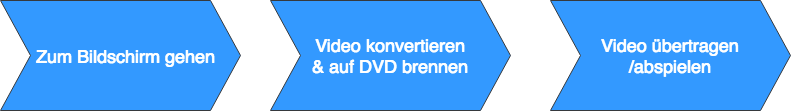
\includegraphics[width=1\textwidth]{images/01_Introduction/WayToDisplay.png}
\caption{Prozess des Anzeigens}
\label{img:processofshow}
\end{figure}

\section{Aufgabenstellung}
Im Rahmen dieser Arbeit war unsere Aufgabenstellung den bestehenden Signage Server um folgende Funktionen zu erweitern:

\begin{enumerate}
	\item {\em Meldungen:} Anzeigen von Meldungen der Schulleitung, um Informationen den Schülern näher zu bringen. 
	\item {\em Slideshow:} Schaffen einer Plattform die es ermöglicht Bilder vom vm59.htl-leonding.ac.at Server über das Signage System anzuzeigen.
	\item {\em Medien abspielen:} Dem Benutzer soll es ermöglicht werden, Medien die auf dem Digital Signage Server liegen auf der gewünschten Anzeige abspielen zu können.
	\item {\em Strukturübersicht:} Roh formatierte Ausgabe der Layouts die sich auf dem Signage Server befinden, um eine Übersicht über die Struktur zu erhalten.	
\end{enumerate}

\section{Ziele}
Ziel ist es, dass aktuelle Nachrichten oder Informationen den Schülern und Schülerinnen der HTL Leonding näher gebracht werden. Diese Nachrichten können verschiedenster Natur sein. Zum Beispiel Ankündigungen, Warnung oder sonstige hilfreiche Informationen.
Der Aufwand für das Erstellen von Slideshows, Informationselementen soll vermindert werden. Es sollen mehrere Datentypen unterstützt werden und auch das Präsentieren von Projekten erleichtert werden.

